\documentclass{beamer}

\useoutertheme[subsection=false]{miniframes}
\usecolortheme{beaver}
\setbeamertemplate{navigation symbols}{}
\setbeamertemplate{footline}{}
\usepackage{graphicx}
\usepackage{url}
\usepackage{datetime}

\newcommand {\framedgraphic}[3] {
  \begin{frame}{#1}
    \vspace{-0.5cm}
    \begin{center}
      \includegraphics[width=0.9\textwidth,keepaspectratio]{#2}
    \end{center}
    \vspace{-1cm}
    \begin{center}
      #3
    \end{center}
  \end{frame}
}
\newcommand{\lectureDate}{\formatdate{04}{10}{2018}}

\setbeamertemplate{caption}{\raggedright\insertcaption\par}
\title{MATH211: Linear Methods I}
\author{Matthew Burke}
\date{\lectureDate}
\begin{document}

\frame{\titlepage}

\begin{frame}{Lecture on \lectureDate}
  \tableofcontents
\end{frame}

\section*{Last time}
\label{sec:Last-time}

\begin{frame}{Last time}
  \begin{itemize}
  \item Cofactor expansion along first row\vfill
  \item Cofactor expansion along arbitrary row or column\vfill
  \item Adjugate matrix
  \end{itemize}
\end{frame}

\section{Adjugates and inverses}

\begin{frame}
  \begin{beamercolorbox}[sep=12pt,center]{part title}
    \usebeamerfont{section title}\insertsection\par
  \end{beamercolorbox}
\end{frame}

\begin{frame}{Adjugate matrix}
  \begin{definition}[Matrix of cofactors]
    \begin{align*}
      cof(A)_{ij} &= cof_{ij}(A)\\
                    &= (-1)^{i+j}minor_{ij}(A)\\
                    &= (-1)^{i+j}\left|A(i|j)\right|
    \end{align*}
  \end{definition}\vfill
  \begin{definition}[Adjugate matrix]
    \begin{align*}
      adj(A)_{ij} &= (cof(A)_{ij})^T\\
                  &= cof_{ji}(A)\\
                  &= (-1)^{j+i}\left|A(j, i)\right|
    \end{align*}
  \end{definition}
\end{frame}

\begin{frame}{Theorems}
  \begin{theorem}[Adjugate is almost inverse]
    \begin{equation*}
      A\cdot adj(A) = adj(A)\cdot A = det(A) I
    \end{equation*}
  \end{theorem}\vfill
  So if $det(A)$ is not $0$ then
  \begin{equation*}
    A^{-1} = \frac{1}{det(A)}adj(A)
  \end{equation*}
  This is not an efficient method to calculate the inverse.
\end{frame}

\begin{frame}{Example}
  \begin{example}
    Find the inverse for
    \begin{equation*}
      \left[
	\begin{array}{ccc}
          4&0&3\\
          1&9&7\\
          0&6&4
	\end{array}
      \right]
    \end{equation*}
    using the adjugate matrix formula.
  \end{example}
\end{frame}

\begin{frame}
  Questions?
\end{frame}

\section{Cramer's rule}

\begin{frame}
  \begin{beamercolorbox}[sep=12pt,center]{part title}
    \usebeamerfont{section title}\insertsection\par
  \end{beamercolorbox}
\end{frame}

\begin{frame}{Using the inverse to solve a system}
  Recall that if $A$ is invertible then
  \begin{equation*}
    Ax=b \implies x = A^{-1}b
  \end{equation*}
  and we can use the formula above to calculate $A^{-1}b$\dots
\end{frame}

\begin{frame}{Using adjugate to solve system}
  \begin{align*}
    x_i &= (A^{-1}b)_{i}\\
        &= \sum_{k=1}^n(A^{-1})_{ik}b_k\\
        &= \sum_{k=1}^n\frac{1}{det(A)}adj(A)_{ik}b_k\\
        &= \frac{1}{det(A)}\sum_{k=1}^nb_k(-1)^{i+k}\left|A(k, i)\right|\\
        &= \frac{1}{det(A)}det(A_i)
  \end{align*}
  where $A_i$ results from replacing the $i$th column of $A$ with $b$.
\end{frame}

\begin{frame}{Cramer's rule}
  If $A$ is invertible then the solutions to
  \begin{equation*}
    A \left[
      \begin{array}{c}
        x_1\\
        x_2\\
        \vdots\\
        x_n
      \end{array}
    \right] = b
  \end{equation*}
  are
  \begin{equation*}
    x_i = \frac{det(A_i)}{det(A)}
  \end{equation*}
  This method of solving systems is usually computationally inefficient.
\end{frame}

\begin{frame}{Example}
  \begin{example}
    Find $x_2$ such that
    \begin{equation*}
      \left[
	\begin{array}{ccc}
          3&1&-1\\
          5&2&0\\
          1&1&-1
	\end{array}
      \right]
      \left[
          \begin{array}{c}
            x_1\\
            x_2\\
            x_3
          \end{array}
        \right]=
        \left[
          \begin{array}{c}
            -1\\
            2\\
            1
          \end{array}
        \right]
    \end{equation*}
  \end{example}
\end{frame}

\begin{frame}
  Questions?
\end{frame}

\section{Common determinants}

\begin{frame}
  \begin{beamercolorbox}[sep=12pt,center]{part title}
    \usebeamerfont{section title}\insertsection\par
  \end{beamercolorbox}
\end{frame}

\begin{frame}{Determinant of product (picture)}
  \hspace{3.1cm}\raisebox{-0.5\height}{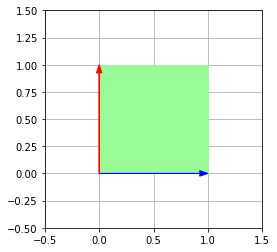
\includegraphics[scale=0.4]{2018-10-04I.png}}$\xrightarrow{B}$
  \raisebox{-0.5\height}{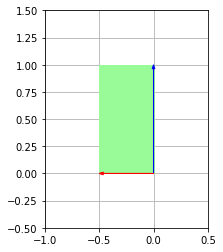
\includegraphics[scale=0.4]{2018-10-04B.png}}\\
  \hspace{-1cm}\raisebox{-0.5\height}{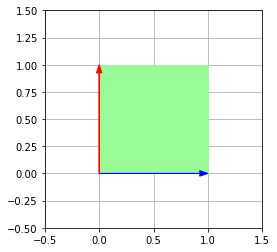
\includegraphics[scale=0.4]{2018-10-04I.png}}$\xrightarrow{A}$
  \raisebox{-0.5\height}{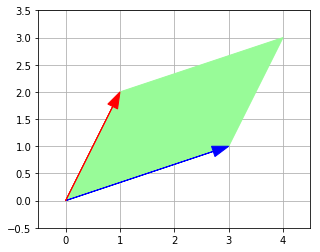
\includegraphics[scale=0.4]{2018-10-04A.png}}$\xrightarrow{B}$
  \raisebox{-0.5\height}{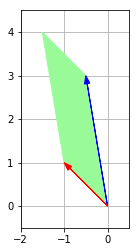
\includegraphics[scale=0.4]{2018-10-04BA.png}}
\end{frame}

\begin{frame}{Determinants and elementary matrices}
  Recall:-\vfill
  \begin{itemize}
  \item Multiplying a row/column by a scalar $k$
    \begin{itemize}
    \item multiplies the determinant by $k$.
    \end{itemize}\vfill
  \item Swapping two rows/columns
    \begin{itemize}
    \item multiplies the determinant by $-1$.
    \end{itemize}\vfill
  \item Adding a multiple of one row/column to another
    \begin{itemize}
    \item has no effect on the determinant.
    \end{itemize}
  \end{itemize}\vfill
  Furthermore each operation can be carried out by multiplying on the left by the corresponding elementary matrix:
  \begin{equation*}
    A \mapsto EA
  \end{equation*}
\end{frame}

\begin{frame}{Determinants and elementary matrices}
  Therefore:\vfill
  \begin{itemize}
  \item if $E$ multiplies a row/column by a scalar $k$
    \begin{itemize}
    \item $det(EA)=k\cdot det(A)$
    \item $det(E)=k$
    \end{itemize}\vfill
  \item if $E$ swaps two rows/columns
    \begin{itemize}
    \item $det(EA) = -det(A)$
    \item $det(E) = -1$
    \end{itemize}\vfill
  \item if $E$ adds a multiple of one row/column to another
    \begin{itemize}
    \item $det(EA) = det(A)$
    \item $det(E) = 1$
    \end{itemize}
  \end{itemize}
\end{frame}

\begin{frame}{Determinant of product (algebra)}
  \begin{lemma}[Determinant of product of elementary matrices]
    If $E$ and $F$ are elementary matrices then
    \begin{equation*}
      det(EF) = det(E)det(F)
    \end{equation*}
  \end{lemma}\vfill
  \begin{theorem}[Determinant of product]
    \begin{equation*}
      det(BA) = det(B)det(A)
    \end{equation*}
    \begin{proof}
      Non-essential exercise. (Divide into cases based on whether $A$ and $B$ are invertible.)
    \end{proof}
  \end{theorem}
\end{frame}

\begin{frame}{Determinant of transpose}
  \begin{theorem}[Determinant of transpose]
    \begin{equation*}
      det(A^T) = det(A)
    \end{equation*}
    \begin{proof}
      The row operations that take $A$ to triangular form have the same effect on the determinant as the column operations that take $A^T$ to triangular form.
    \end{proof}
  \end{theorem}
\end{frame}

\begin{frame}{Determinant of inverse and adjugate}
  \begin{theorem}[Determinant of inverse]
    If $A$ is invertible then
    \begin{equation*}
      det(A^{-1}) = \frac{1}{det(A)}
    \end{equation*}
    \begin{proof}
      Check for elementary matrices. Then express $A$ in terms of elementary matrices.
    \end{proof}
  \end{theorem}
  \begin{theorem}[Determinant of adjugate]
    For any square matrix $A$
    \begin{equation*}
      det(adj(A)) = (det(A))^{n-1}
    \end{equation*}
  \end{theorem}
\end{frame}

\begin{frame}{Examples}
  \begin{example}
    Find
    \begin{equation*}
      \left|
        \left[
          \begin{array}{cc}
            2&3\\
            4&5
          \end{array}
        \right]
        \left[
          \begin{array}{cc}
            1&1\\
            1&1
          \end{array}
        \right]
      \right|
    \end{equation*}
  \end{example}
  \begin{example}
    Find
    \begin{equation*}
      \left|
        \left[
          \begin{array}{cc}
            0&1\\
            1&0
          \end{array}
        \right]
        \left[
          \begin{array}{cc}
            5&4\\
            -3&8
          \end{array}
        \right]
      \right|
    \end{equation*}
  \end{example}
\end{frame}

\begin{frame}{Examples}
  \begin{example}
    Suppose $A$, $B$ and $C$ are $4\times 4$ matrices with
    \[ \det A = -1, \det B = 2, \mbox{ and } \det C=1.\]
    Find $\det(2A^2(B^{-1})(C^T)^3 B(A^{-1}))$.
  \end{example}
  \begin{example}
    Suppose $A$ is a $3\times 3$ matrix.
    Find $\det A$ and $\det B$ if
    \[ \det(2A^{-1})=-4=\det(A^3(B^{-1})^T).\]
  \end{example}
\end{frame}

\begin{frame}
  Questions?
\end{frame}

\section{Polynomial interpolation}

\begin{frame}
  \begin{beamercolorbox}[sep=12pt,center]{part title}
    \usebeamerfont{section title}\insertsection\par
  \end{beamercolorbox}
\end{frame}

\begin{frame}{Example}
  \begin{example}
    Given data points $(0,1)$, $(1,2)$, $(2,5)$ and $(3,10)$,
    find an interpolating polynomial 
    $p(x)$ of degree at most three, 
    and then estimate the value of $y$ corresponding to $x=\frac{3}{2}$.
  \end{example}
\end{frame}

\begin{frame}{General theory}
  If $x_1$, $x_2$, \dots, $x_n$ are all distinct then
  \begin{equation*}
    \left|
      \begin{array}{cccccc}
        1&x_1&x_1^2&x_1^3&\dots&x_1^n\\
        1&x_2&x_2^2&x_2^3&\dots&x_2^n\\
        \dots&\dots&\dots&\dots&\dots&\dots\\
        1&x_n&x_n^2&x_n^3&\dots&x^n
      \end{array}
    \right|
  \end{equation*}
  is non-zero.
\end{frame}

\begin{frame}
  Questions?
\end{frame}

\end{document}